To motivate the need for coordination, we use the Single Source Shortest
Path~(SSSP) program, a concise program that, as we will see, can take advantage
of custom scheduling policies to improve its performance.
Figure~\ref{code:shortest_path_program} and Figure~\ref{code:coord:sssp_init}
shows a possible implementation in LM, and Fig.~\ref{fig:shortest_path_program}
shows an instance of the program on a particular dataset. Note that in
Section~\ref{section:implementation:performance}, we presented the
MSSD program which is essentially the SSSP program modified to compute multiple
shortest distances.

The SSSP program starts with the declaration of the predicates~
(lines~\ref{line:coord:sssp_pred1}-\ref{line:coord:sssp_pred2}). As usual, the
\code{edge} predicate is a persistent predicate that describes the edges of the
graph, where the third argument is the weight of each edge. Predicate
\code{shortest} represents a valid distance and path from node \code{@1} to the
node in the first argument.  Predicate \code{relax} also represents a valid
path, and, is used to improve the distance in \code{shortest}.  The program
computes the shortest distance from node \code{@1} by improving the distance in
the \code{shortest} facts, until the shortest distance is reached in all nodes.
In Fig.~\ref{code:coord:sssp_init}, we declare an example set of initial facts
for the program: \code{edge} facts describe the graph; \code{shortest(A, +00,
[])} is the initial shortest distance (infinity) for all nodes; and
\code{relax(@1, 0, [@1])} starts the algorithm by setting the distance from
\code{@1} to \code{@1} to be 0.

\begin{figure}[ht]
\begin{LineCode}[commandchars=\*\#\&]
type edge(node, node, int).*label#line:coord:sssp_pred1&*hfill// Predicate declaration
type linear shortest(node, int, list int).
type linear relax(node, int, list int).*label#line:coord:sssp_pred2&

shortest(A, D1, P1), D1 > D2, relax(A, D2, P2)*label#line:coord:sssp_first1&*hfill// Rule 1: newly improved path
   -o shortest(A, D2, P2),
      {B, W | !edge(A, B, W) -o relax(B, D2 + W, P2 ++ [B])}.*label#line:coord:sssp_first2&

shortest(A, D1, P1), D1 <= D2, relax(A, D2, P2)*label#line:coord:sssp_second1&*hfill// Rule 2: longer path
   -o shortest(A, D1, P1).*label#line:coord:sssp_second2&
\end{LineCode}
\mycap{Single Source Shortest Path program code.}
\label{code:shortest_path_program}
\end{figure}

\begin{figure}[ht]
\begin{LineCode}[commandchars=\*\#\&]
!edge(@1, @2, 3). !edge(@1, @3, 1).
!edge(@3, @2, 1). !edge(@3, @4, 5).
!edge(@2, @4, 1).
shortest(A, +00, []).
relax(@1, 0, [@1]).
\end{LineCode}
\mycap{Initial facts for the SSSP program.}
\label{code:coord:sssp_init}
\end{figure}

\iffalse
\begin{figure}[ht]
\begin{LineCode}[commandchars=\*\#\&]
!edge(@1, @2, 3). !edge(@1, @3, 1).
!edge(@3, @2, 1). !edge(@3, @4, 5).
!edge(@2, @4, 1).
shortest(@1, 0, []).
shortest(@2, 2, [@1, @3, @2]).
shortest(@3, 1, [@1, @3]).
shortest(@4, 3, [@1, @3, @2, @4]).
\end{LineCode}
\mycap{Final database of facts for the SSSP program.}
\label{code:coord:sssp_end}
\end{figure}
\fi
\begin{figure}
\begin{center}
   \begin{subfigure}[b]{0.49\textwidth}
      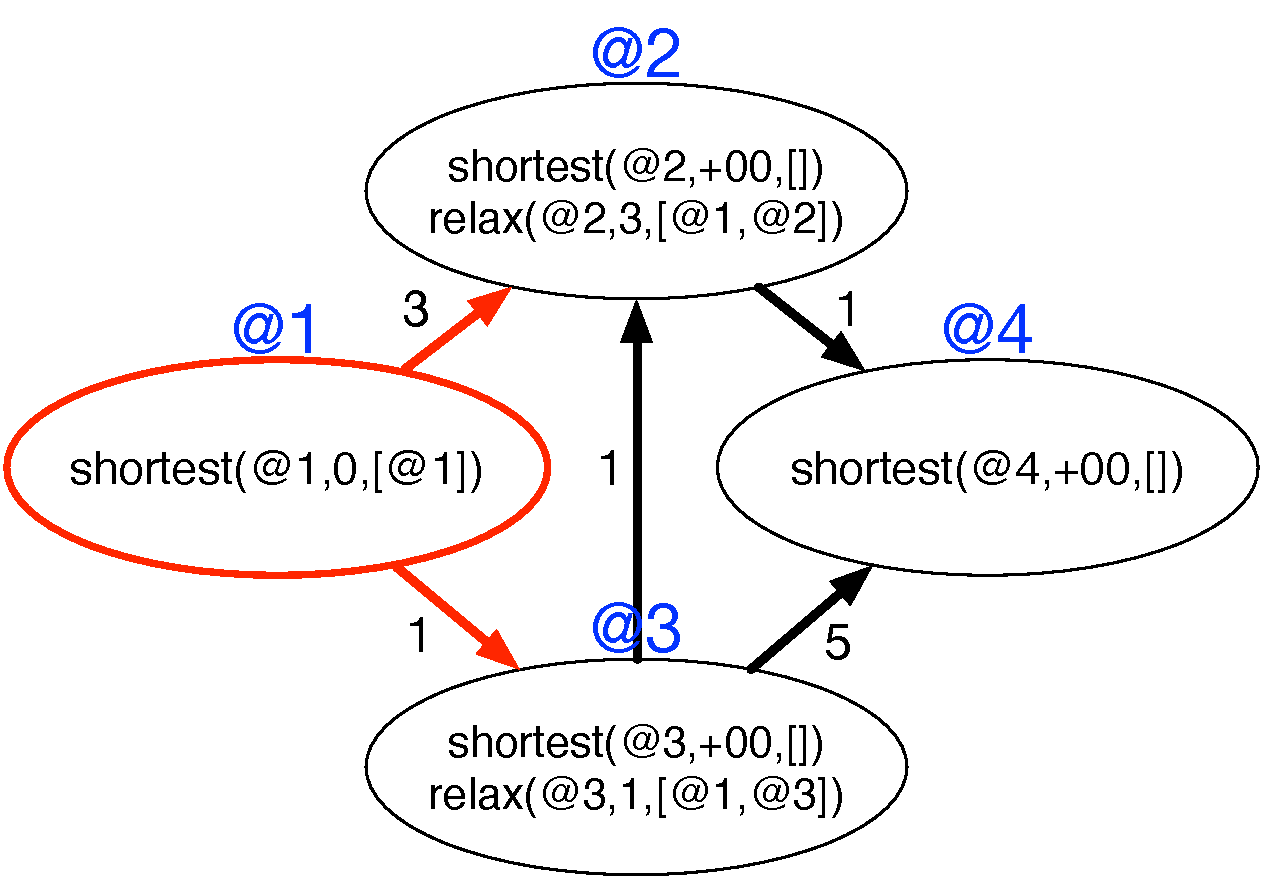
\includegraphics[width=\textwidth]{figures/sssp/shortest2}
      \mycap{}
   \end{subfigure}
   \begin{subfigure}[b]{0.49\textwidth}
      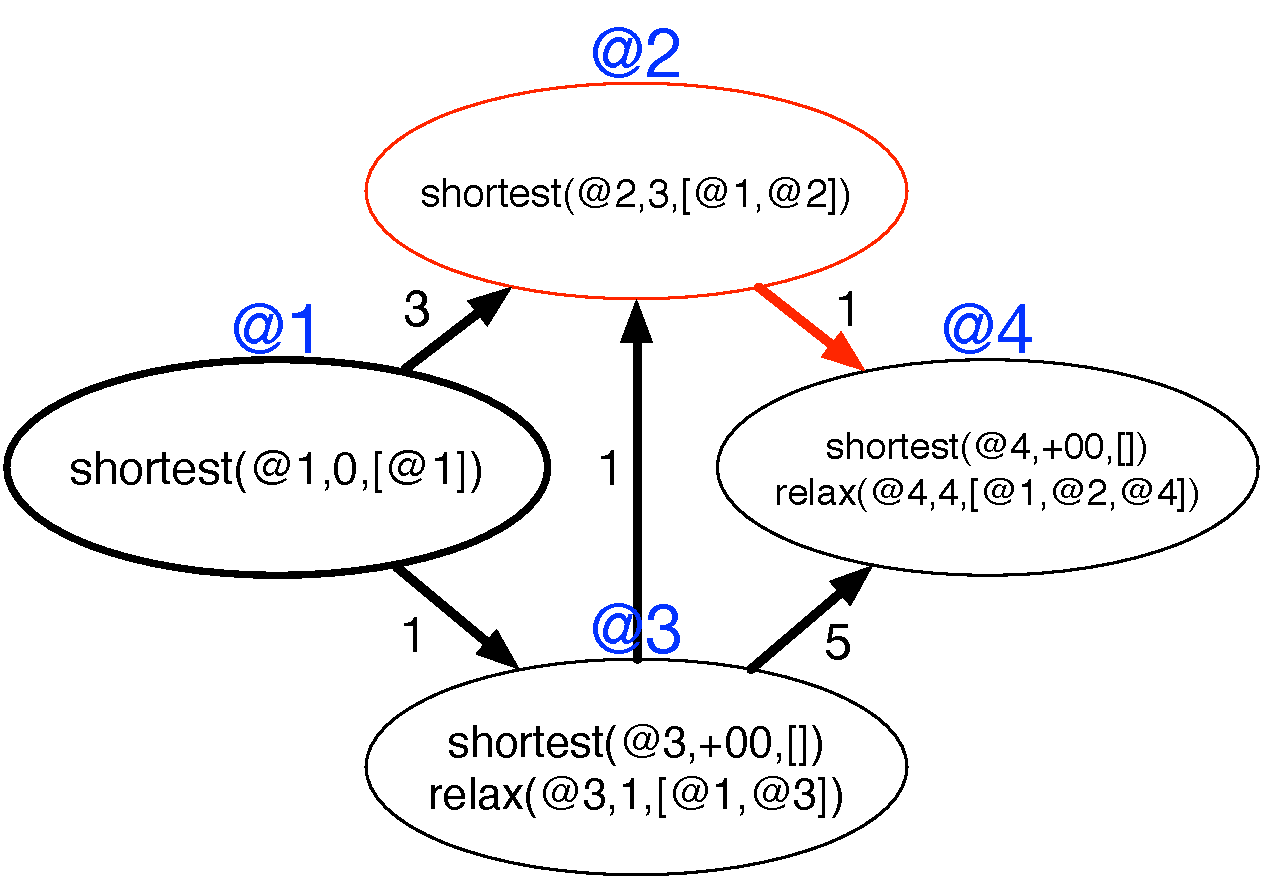
\includegraphics[width=\textwidth]{figures/sssp/shortest3}
      \mycap{}
   \end{subfigure}
   \begin{subfigure}[b]{0.49\textwidth}
      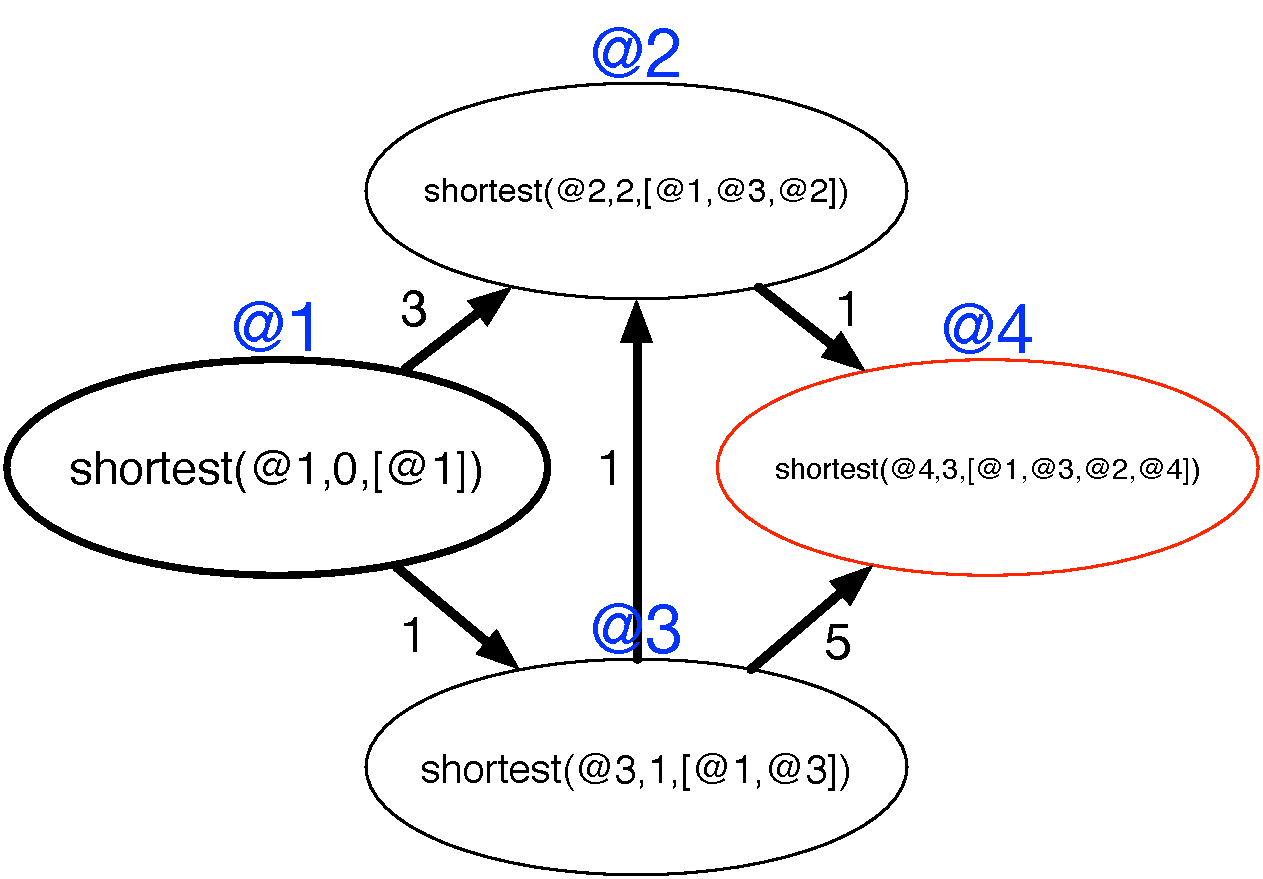
\includegraphics[width=\textwidth]{figures/sssp/shortest8}
      \mycap{}
   \end{subfigure}
\end{center}

\mycap{Graphical representation of an example dataset for the SSSP program: (a) represents the
   program's state after propagating the initial distance at node \code{@1}, followed by (b)
   where the first rule is applied in node \code{@2}, and (c) represents the
   final state of the program, where all the shortest paths have been computed.}

\label{fig:shortest_path_program}
\end{figure}

The first rule of the program
(lines~\ref{line:coord:sssp_first1}-\ref{line:coord:sssp_first2}) reads as
follows: if the current \code{shortest} path \code{P1} with distance \code{D1}
is larger than a new path \code{relax} with distance \code{D2}, then replace the
current shortest path with \code{D2}, delete the new \code{relax} path and
propagate new paths to the neighbors (comprehension at
line~\ref{line:coord:sssp_first2}). The comprehension iterates over the edges of
node \code{A} and derives a new \code{relax} fact for each node \code{B} with
the distance \code{D2 + W}, where \code{W} is the weight of the edge. For
example, in Fig.~\ref{fig:shortest_path_program}~(a) we apply rule 1 in node
\code{@1} and two new \code{relax} facts are derived at node \code{@2} and
\code{@3}.  Fig.~\ref{fig:shortest_path_program}~(b) is the result after
applying the same rule but at node \code{@2}.

The second rule of the program
(lines~\ref{line:coord:sssp_second1}-\ref{line:coord:sssp_second2}) retracts a
\code{relax} fact that has a longer distance than the current shortest distance
stored in \code{shortest}. There are many opportunities for custom scheduling
in the SSSP program. For instance, after applying rule 1 in
Fig.~\ref{fig:shortest_path_program}~(a), it is possible to either apply rules
in either node \code{@2} or node \code{@3}.  This decision depends largely on
implementation factors such as node partitioning and number of threads in the
system. Still, it is easy to prove that, independent of the particular scheduling used, the final
result presented in Fig.~\ref{fig:shortest_path_program}~(c) is always achieved.

The SSSP program is concise and declarative but its performance depends on the
order in which nodes are executed. If nodes with greater distances are
prioritized over other nodes, the program will generate more \code{relax} facts
and it will take longer to reach the shortest distances. From
Fig.~\ref{fig:shortest_path_program}, it is clear that the best scheduling is
the following: \code{@1}, \code{@3}, \code{@2} and then \code{@4}, where only 4
\code{relax} facts are generated. If we had decided to process nodes in order
\code{@1}, \code{@2}, \code{@4}, \code{@3}, \code{@4}, \code{@2}, then 6
\code{relax} facts would have been generated.  The optimal solution for SSSP is
to schedule the node with the shortest distance, which is essentially the
Dijkstra shortest path algorithm~\cite{Dijkstra}. Note how it is possible to
change the complexity of the algorithm by simply changing the order of node
computation, but still retain the same declarative nature of the program.

